\documentclass[12pt]{article}
\usepackage{float}
\usepackage{graphicx}
\usepackage{fontspec}
\usepackage{titlesec}
\usepackage{setspace}
\usepackage[style=numeric,backend=biber,sorting=none]{biblatex}
\usepackage[a4paper, total={6in, 8in}, margin=0.5in]{geometry}
\addbibresource{ref.bib}

%%%%%%%% FORMAT
\singlespacing
\setmainfont{Arial}

\titleformat*{\section}{\normalsize\bfseries}
\titleformat*{\subsection}{\normalsize\bfseries}

\pagenumbering{gobble} % Suppress page number

% \titlespacing\section{0pt}{12pt plus 4pt minus 2pt}{0pt plus 2pt minus 2pt}
% \titlespacing\subsection{0pt}{12pt plus 4pt minus 2pt}{0pt plus 2pt minus 2pt}
% \titlespacing\subsubsection{0pt}{12pt plus 4pt minus 2pt}{0pt plus 2pt minus 2pt}


\begin{document}
  
%%%%%%%%% TITLE  
\title{\large Give a brief comparison on the innate and the adaptive defence systems \vspace{-2em}}
% \author{\large Yujia Shi\vspace{-1em}}
\date{\vspace{-2.5em}}
\maketitle

%%%%%%%%% BODY TEXT
\section{INTROUDCTION}

Our living environment is heavily filled with pathogenic and non-pathogenic microbes which includes a variety of toxic and allergenic substances to pose threat to normal homeostasis by replicating, spreading, and threatening normal host functions. To recognize and destroy those abnormal cells in our body, the immune system is designed and evolved to defense against dangerous invaders such as gerns, virus, cancer cells, and organs and tissues transplanted, at the same time, they also avoid the immune system cause enormous destruction on self-tissue that might eliminate 
commensal microbes by detecting the mark of toxin it is distinct from host cells or the structural features of the pathogen.\medskip

The immune system is a complex protective network consist of white blood cells, antibodies, the complement system, the lymphatic system. Each of these elements is important to the immune system, particularly for bone marrow and thymus. Both bone marrow and thymus have belonged to primary lymphoid organs were to generate and multiply two main lymphocytes, which include B and T cells.
Bone marrow is a spongy tissue responsible to produce all body's blood cells, including B (mature in bond marrow) and T lymphocytes(mature in thymus). Different blood cells will work together within the immune system and move to place needed to defense foreign substances in the body from the bone marrow; while the Thymus is a gland that can be found above the heart and between the lungs. The Thymus eventually will be replaced by connective tissue and fat, which only active in the stage of puberty and gradually slow down. The thymus is taking charge of producing the hormone thymosin, and thereby assist in the generation of T cells.T cells are born in the bone marrow and mature in the thymus, after multiplying in the thymus which will differentiate into helper, regulatory,  cytotoxic and memory T cells with different functions such as 
\begin{itemize}
    \item [1)] 
    CD4+ helper T cells: Be helper cells to guide the immune system to attack invaders as rapidly and efficiently as possible, which also communicate with the B cells to produce antibodies.
    \item [2)]
    CD8+ killer T cells: Their daily routine work is direct destroys countless cancer and virus-infected cells in the body. and equipped with the ability to distinguish the difference between foreign molecules and the body's own antigens.
    \item [3)]
    Cytotoxic T cells:
    The cytotoxic cell is a type of white blood cell that is the main effector in the adaptive immune system and is primarily activated by cytokines, so they can kill cells that are infected with virus or bacteria, cancer cells.
    \item [4)]
    Regulatory T cell:
    Regulatory T cell, also called Tregs, is capable of regulating and suppressing harmful cells, they are the key components that help to prevent excessive immune response and autoimmune disease.
\end{itemize}
and equipped with the ability to distinguish the difference between foreign molecules and the body's own antigens. T cells can identify self-structures and foreign antigens make it become an critical elegant mechanism in the immune system. Apart from the tissue and organs component of bone marrow and thymus, other components comprised in the immune system also play a critical role in making the system works smoothly is capable of activating and mobilizing forces to prevent any potentially harmful substances such as toxic or allergenic substances enter through our mucosal surface..\medskip

Before taking action to respond and control the pathogen microbes, toxin, and exogenous threats, it is important for the immune system to initiate the mechanisms of self-nonself recognition, to differentiate self from non-self, in other words, is to distinguish the antigens belong in our body from foreign antigens such as toxins, chemicals, drugs which may be evoking the immune system called immunogens. The mechanisms of discrimination of self from non-self are not only facilitated the process to destroy or clear up a board range of harmful microbial cells, toxic and allergenic substances but also to avoid these destructive mechanisms damage mammalian host's own tissue, resulting in a broad class of autoimmune disorders.\medskip

The antigen is a complex nature of protein substances that will bind particularly to a receptor molecule and made by the body's infection-fighting white blood cells(lymphocytes). Antigenes with molecules can be found in several places such as viruses, bacteria, and fungi, sometimes located on the surface of foreign substances, such as dust and organ transplantation. An antigen may or may not stimulate an immune response, especially activating lymphocytes when it binds to a receptor molecule, even though antigenes usually have a diversity of three-dimensional patterns on distinct places of their surfaces and each pattern such as an antigenic determinant, or epitope has the ability to stimulate different lymphocyte receptor to multiply and initiate the immune response, for example, the generation of antibodies or the activation of cytotoxic cells. Although the truth that some antigenes can not evoke the immune system by themselves, still helpful in the study of an immune response, as they can join with other larger and more complex protein molecules to become immunogenic. Generally speaking, antigens can be divide into two main divisions: foreign(or heteroantigens) and antigenes. 
Foreign antigens are coming from the outside of the body, there are a variety of substances can be classified into foreign antigens, example includes the substance generated from virus, bacterial and protozoa, some of the protein in foods, the serum and red blood cells components from other people. In contrast to foreign antigens, Autoantigens resides within the body.\medskip

In general, an individual without autoimmune disorders, his or her body can carry out the process of discriminating self from no-self by inducing the immune system to generate the autoantibodies or destroy the antigen directly, which is called an immunogen.


 \begin{figure}[H]
    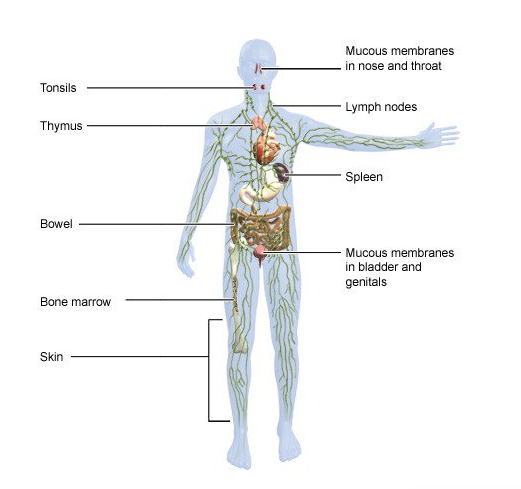
\includegraphics[width=0.7 \linewidth,height=0.62 \columnwidth]{/Users/yu-pinglin/Desktop/Essay/6001_Francis.png}
    \centering
    \caption{The 4 pillars for building a sustainable portfolio of
    core facilities.}
\end{figure}

\section{The innate and adaptive immune systems}
The immune response is made up of two parts: the innate (non-specialized) immunity and the adaptive (specialized) immunity. The innate immune response to an invader fast-acting and non-specific, which is the immunity that a person is born with, while for adaptive immunity which is not as immediate as innate immunity, this type of immunity is usually slow to respond to a new invader at the very beginning. Lymphocytes are the type of white blood cell (B and T cells) take charge of adaptive immunity, when they first encounter foreign substances (antigens), they need time to learn, adapt and remember. The components of adaptive immunity will learn the best way to attack each invader and begin to establish a memory for that invader. Thereafter, the response will be improved because the memory is formed for the past invader, so B and T cells can identify previously encountered invaders in the shortest of time, working together to destroy it even more efficiently.\medskip

People usually describe the innate and adaptive immune system as contrasting, separate arms of the host response; however, these two systems cooperate and work on different tasks.

\subsection{Innate defence system}
The innate immune system offers a first-line barrier and non-specific response to keep potential pathogens, which includes viruses, bacteria, fungi, protozoans, and worm from entering your body. It acts very quickly to prevent the transmission and movement of germs and foreign substances throughout the body. For example, the innate system will destroy bacteria within a few hours, when it has entered the skin via a small wound. The reason why the innate system is referred to as a "nonspecific" immune system is that it responds in the same way to the specified virus and bacterial that it recognizes. The innate immune system provides nonspecific defense protection which is made up of several defense mechanisms, which include Physical barriers, Chemical barriers, and Cellular defenses.
\begin{itemize}
    \item [1)] 
    Physical barriers: All outer and inner surfaces of our body are belong to the physical
    barriers, which is the first line of defense in fighting invasion by microbes and parasites. These include the skin and mucous membranes. Human skin includes an outer layer of the cell which is considered as a mechanical barrier to infection. Furthermore, the skin gland will secrete a variety of chemicals substances, or enzymes, for example, secrete oleic acid to kill bacterial or lysozyme to destroy the outer wall of bacterial. There is a variety of mucous membranes that surround our body organs, to protect the body from being infected and keep those tissue moisturized by secreting mucus.
    \item [2)]
    Chemical barriers: The primary function of chemical barriers such as tears, mucous and stomach acid, is to harm and destroy the invader which about to enter the internal tissues.
    \item [3)]
    Cellular barriers: The cellular in the innate immune system are nonspecific effectors cells such as scavenger cells and natural killer cells, they will neutralize or destroy those pathogens and substances that are likely dangerous to our body. 
\end{itemize}

\subsection{Adaptive defence system}
The adaptive defense system will be becoming a prominent defense after the first line of host defense.
The second line of protection is called adaptive immunity, we also referred it as acquired immunity or specific immunity, and is only found in vertebrates and will not always exist throughout an individual's entire lifespan. It is much slower to respond than the innate immunity response. the adaptive immune response is the clone expansion of T and B cells, which takes the body time to increase the number of T and lymphocytes. However, it is more accurate and robust than the innate immune system, the adaptive immune system can respond faster when an individual met some pathogen for the second time. The increased speed is due to memory cells. 

\subsection{Innate vs adaptive immunity}
Give a comparison between innate and adaptive defense system. The innate immune response is immediate with limited power to stop the spread of germs. the adaptive immune response is particularly specific, long-term(over 96 hours).In terms of the cell types involved in both immunity are different. In the innate immune response which includes macrophages, neutrophils, eosinophils; while for adaptive immune response are based primarily on the antigen-specific receptors of T- and B-lymphocytes.

\section{CONCLUSION}
The immune system consists of many components such as cellular components, molecular components to protect us from a universe of pathogenic microbes. Understanding the function of different components will allow for improvement in vaccines, immunomodulatory therapeutics as well as avoidance of unexpected tissue injury.


\emergencystretch=1em
\printbibliography[title=Reference]

\end{document}




